\documentclass[10pt, aspectratio=169]{beamer}















\usepackage[breakable]{tcolorbox}
% Basic figure setup, for now with no caption control since it's done
% automatically by Pandoc (which extracts ![](path) syntax from Markdown).
\usepackage{graphicx}
% Maintain compatibility with old templates. Remove in nbconvert 6.0
\let\Oldincludegraphics\includegraphics
% Ensure that by default, figures have no caption (until we provide a
% proper Figure object with a Caption API and a way to capture that
% in the conversion process - todo).
\usepackage{caption}
% \DeclareCaptionFormat{nocaption}{}
% \captionsetup{format=nocaption,aboveskip=0pt,belowskip=0pt}

\usepackage[Export]{adjustbox} % Used to constrain images to a maximum size
\adjustboxset{max size={0.9\linewidth}{0.9\paperheight}}
\usepackage{float}
\floatplacement{figure}{H} % forces figures to be placed at the correct location
\usepackage{xcolor} % Allow colors to be defined
\usepackage{enumerate} % Needed for markdown enumerations to work
\usepackage{geometry} % Used to adjust the document margins
\usepackage{amsmath} % Equations
\usepackage{amssymb} % Equations
\usepackage{textcomp} % defines textquotesingle
% Hack from http://tex.stackexchange.com/a/47451/13684:
\AtBeginDocument{%
\def\PYZsq{\textquotesingle}% Upright quotes in Pygmentized code
}
\usepackage{upquote} % Upright quotes for verbatim code
\usepackage{eurosym} % defines \euro
\usepackage[mathletters]{ucs} % Extended unicode (utf-8) support
\usepackage{fancyvrb} % verbatim replacement that allows latex
\usepackage{grffile} % extends the file name processing of package graphics
		 % to support a larger range
\makeatletter % fix for grffile with XeLaTeX
\def\Gread@@xetex#1{%
\IfFileExists{"\Gin@base".bb}%
{\Gread@eps{\Gin@base.bb}}%
{\Gread@@xetex@aux#1}%
}
\makeatother

% The hyperref package gives us a pdf with properly built
% internal navigation ('pdf bookmarks' for the table of contents,
% internal cross-reference links, web links for URLs, etc.)
\usepackage{hyperref}
% The default LaTeX title has an obnoxious amount of whitespace. By default,
% titling removes some of it. It also provides customization options.
%\usepackage{titling}
\usepackage{longtable} % longtable support required by pandoc >1.10
\usepackage{booktabs}  % table support for pandoc > 1.12.2
%\usepackage[inline]{enumitem} % IRkernel/repr support (it uses the enumerate* environment)
%\usepackage[normalem]{ulem} % ulem is needed to support strikethroughs (\sout) normalem makes italics be italics, not underlines
%\usepackage{mathrsfs}
% Colors for the hyperref package
\definecolor{urlcolor}{rgb}{0,.145,.698}
\definecolor{linkcolor}{rgb}{0,0.0}
\definecolor{citecolor}{rgb}{.12,.54,.11}

% ANSI colors
\definecolor{ansi-black}{HTML}{3E424D}
\definecolor{ansi-black-intense}{HTML}{282C36}
\definecolor{ansi-red}{HTML}{E75C58}
\definecolor{ansi-red-intense}{HTML}{B22B31}
\definecolor{ansi-green}{HTML}{00A250}
\definecolor{ansi-green-intense}{HTML}{007427}
\definecolor{ansi-yellow}{HTML}{DDB62B}
\definecolor{ansi-yellow-intense}{HTML}{B27D12}
\definecolor{ansi-blue}{HTML}{208FFB}
\definecolor{ansi-blue-intense}{HTML}{0065CA}
\definecolor{ansi-magenta}{HTML}{D160C4}
\definecolor{ansi-magenta-intense}{HTML}{A03196}
\definecolor{ansi-cyan}{HTML}{60C6C8}
\definecolor{ansi-cyan-intense}{HTML}{258F8F}
\definecolor{ansi-white}{HTML}{C5C1B4}
\definecolor{ansi-white-intense}{HTML}{A1A6B2}
\definecolor{ansi-default-inverse-fg}{HTML}{FFFFFF}
\definecolor{ansi-default-inverse-bg}{HTML}{000000}

% commands and environments needed by pandoc snippets
% extracted from the output of `pandoc -s`
\providecommand{\tightlist}{%
\setlength{\itemsep}{0pt}\setlength{\parskip}{0pt}}
\DefineVerbatimEnvironment{Highlighting}{Verbatim}{commandchars=\\\{\}}
% Add ',fontsize=\small' for more characters per line
\newenvironment{Shaded}{}{}
\newcommand{\KeywordTok}[1]{\textcolor[rgb]{0.00,0.44,0.13}{\textbf{{#1}}}}
\newcommand{\DataTypeTok}[1]{\textcolor[rgb]{0.56,0.13,0.00}{{#1}}}
\newcommand{\DecValTok}[1]{\textcolor[rgb]{0.25,0.63,0.44}{{#1}}}
\newcommand{\BaseNTok}[1]{\textcolor[rgb]{0.25,0.63,0.44}{{#1}}}
\newcommand{\FloatTok}[1]{\textcolor[rgb]{0.25,0.63,0.44}{{#1}}}
\newcommand{\CharTok}[1]{\textcolor[rgb]{0.25,0.44,0.63}{{#1}}}
\newcommand{\StringTok}[1]{\textcolor[rgb]{0.25,0.44,0.63}{{#1}}}
\newcommand{\CommentTok}[1]{\textcolor[rgb]{0.38,0.63,0.69}{\textit{{#1}}}}
\newcommand{\OtherTok}[1]{\textcolor[rgb]{0.00,0.44,0.13}{{#1}}}
\newcommand{\AlertTok}[1]{\textcolor[rgb]{1.00,0.00,0.00}{\textbf{{#1}}}}
\newcommand{\FunctionTok}[1]{\textcolor[rgb]{0.02,0.16,0.49}{{#1}}}
\newcommand{\RegionMarkerTok}[1]{{#1}}
\newcommand{\ErrorTok}[1]{\textcolor[rgb]{1.00,0.00,0.00}{\textbf{{#1}}}}
\newcommand{\NormalTok}[1]{{#1}}

% Additional commands for more recent versions of Pandoc
\newcommand{\ConstantTok}[1]{\textcolor[rgb]{0.53,0.00,0.00}{{#1}}}
\newcommand{\SpecialCharTok}[1]{\textcolor[rgb]{0.25,0.44,0.63}{{#1}}}
\newcommand{\VerbatimStringTok}[1]{\textcolor[rgb]{0.25,0.44,0.63}{{#1}}}
\newcommand{\SpecialStringTok}[1]{\textcolor[rgb]{0.73,0.40,0.53}{{#1}}}
\newcommand{\ImportTok}[1]{{#1}}
\newcommand{\DocumentationTok}[1]{\textcolor[rgb]{0.73,0.13,0.13}{\textit{{#1}}}}
\newcommand{\AnnotationTok}[1]{\textcolor[rgb]{0.38,0.63,0.69}{\textbf{\textit{{#1}}}}}
\newcommand{\CommentVarTok}[1]{\textcolor[rgb]{0.38,0.63,0.69}{\textbf{\textit{{#1}}}}}
\newcommand{\VariableTok}[1]{\textcolor[rgb]{0.10,0.09,0.49}{{#1}}}
\newcommand{\ControlFlowTok}[1]{\textcolor[rgb]{0.00,0.44,0.13}{\textbf{{#1}}}}
\newcommand{\OperatorTok}[1]{\textcolor[rgb]{0.40,0.40,0.40}{{#1}}}
\newcommand{\BuiltInTok}[1]{{#1}}
\newcommand{\ExtensionTok}[1]{{#1}}
\newcommand{\PreprocessorTok}[1]{\textcolor[rgb]{0.74,0.48,0.00}{{#1}}}
\newcommand{\AttributeTok}[1]{\textcolor[rgb]{0.49,0.56,0.16}{{#1}}}
\newcommand{\InformationTok}[1]{\textcolor[rgb]{0.38,0.63,0.69}{\textbf{\textit{{#1}}}}}
\newcommand{\WarningTok}[1]{\textcolor[rgb]{0.38,0.63,0.69}{\textbf{\textit{{#1}}}}}


% Define a nice break command that doesn't care if a line doesn't already
% exist.
\def\br{\hspace*{\fill} \\* }
% Math Jax compatibility definitions
\def\gt{>}
\def\lt{<}
\let\Oldtex\TeX
\let\Oldlatex\LaTeX
\renewcommand{\TeX}{\textrm{\Oldtex}}
\renewcommand{\LaTeX}{\textrm{\Oldlatex}}
% Document parameters
% Document title
%\title{tarantino\_profanity}





% Pygments definitions
\makeatletter
\def\PY@reset{\let\PY@it=\relax \let\PY@bf=\relax%
    \let\PY@ul=\relax \let\PY@tc=\relax%
    \let\PY@bc=\relax \let\PY@ff=\relax}
\def\PY@tok#1{\csname PY@tok@#1\endcsname}
\def\PY@toks#1+{\ifx\relax#1\empty\else%
    \PY@tok{#1}\expandafter\PY@toks\fi}
\def\PY@do#1{\PY@bc{\PY@tc{\PY@ul{%
    \PY@it{\PY@bf{\PY@ff{#1}}}}}}}
\def\PY#1#2{\PY@reset\PY@toks#1+\relax+\PY@do{#2}}

\expandafter\def\csname PY@tok@w\endcsname{\def\PY@tc##1{\textcolor[rgb]{0.73,0.73,0.73}{##1}}}
\expandafter\def\csname PY@tok@c\endcsname{\let\PY@it=\textit\def\PY@tc##1{\textcolor[rgb]{0.25,0.50,0.50}{##1}}}
\expandafter\def\csname PY@tok@cp\endcsname{\def\PY@tc##1{\textcolor[rgb]{0.74,0.48,0.00}{##1}}}
\expandafter\def\csname PY@tok@k\endcsname{\let\PY@bf=\textbf\def\PY@tc##1{\textcolor[rgb]{0.00,0.50,0.00}{##1}}}
\expandafter\def\csname PY@tok@kp\endcsname{\def\PY@tc##1{\textcolor[rgb]{0.00,0.50,0.00}{##1}}}
\expandafter\def\csname PY@tok@kt\endcsname{\def\PY@tc##1{\textcolor[rgb]{0.69,0.00,0.25}{##1}}}
\expandafter\def\csname PY@tok@o\endcsname{\def\PY@tc##1{\textcolor[rgb]{0.40,0.40,0.40}{##1}}}
\expandafter\def\csname PY@tok@ow\endcsname{\let\PY@bf=\textbf\def\PY@tc##1{\textcolor[rgb]{0.67,0.13,1.00}{##1}}}
\expandafter\def\csname PY@tok@nb\endcsname{\def\PY@tc##1{\textcolor[rgb]{0.00,0.50,0.00}{##1}}}
\expandafter\def\csname PY@tok@nf\endcsname{\def\PY@tc##1{\textcolor[rgb]{0.00,0.00,1.00}{##1}}}
\expandafter\def\csname PY@tok@nc\endcsname{\let\PY@bf=\textbf\def\PY@tc##1{\textcolor[rgb]{0.00,0.00,1.00}{##1}}}
\expandafter\def\csname PY@tok@nn\endcsname{\let\PY@bf=\textbf\def\PY@tc##1{\textcolor[rgb]{0.00,0.00,1.00}{##1}}}
\expandafter\def\csname PY@tok@ne\endcsname{\let\PY@bf=\textbf\def\PY@tc##1{\textcolor[rgb]{0.82,0.25,0.23}{##1}}}
\expandafter\def\csname PY@tok@nv\endcsname{\def\PY@tc##1{\textcolor[rgb]{0.10,0.09,0.49}{##1}}}
\expandafter\def\csname PY@tok@no\endcsname{\def\PY@tc##1{\textcolor[rgb]{0.53,0.00,0.00}{##1}}}
\expandafter\def\csname PY@tok@nl\endcsname{\def\PY@tc##1{\textcolor[rgb]{0.63,0.63,0.00}{##1}}}
\expandafter\def\csname PY@tok@ni\endcsname{\let\PY@bf=\textbf\def\PY@tc##1{\textcolor[rgb]{0.60,0.60,0.60}{##1}}}
\expandafter\def\csname PY@tok@na\endcsname{\def\PY@tc##1{\textcolor[rgb]{0.49,0.56,0.16}{##1}}}
\expandafter\def\csname PY@tok@nt\endcsname{\let\PY@bf=\textbf\def\PY@tc##1{\textcolor[rgb]{0.00,0.50,0.00}{##1}}}
\expandafter\def\csname PY@tok@nd\endcsname{\def\PY@tc##1{\textcolor[rgb]{0.67,0.13,1.00}{##1}}}
\expandafter\def\csname PY@tok@s\endcsname{\def\PY@tc##1{\textcolor[rgb]{0.73,0.13,0.13}{##1}}}
\expandafter\def\csname PY@tok@sd\endcsname{\let\PY@it=\textit\def\PY@tc##1{\textcolor[rgb]{0.73,0.13,0.13}{##1}}}
\expandafter\def\csname PY@tok@si\endcsname{\let\PY@bf=\textbf\def\PY@tc##1{\textcolor[rgb]{0.73,0.40,0.53}{##1}}}
\expandafter\def\csname PY@tok@se\endcsname{\let\PY@bf=\textbf\def\PY@tc##1{\textcolor[rgb]{0.73,0.40,0.13}{##1}}}
\expandafter\def\csname PY@tok@sr\endcsname{\def\PY@tc##1{\textcolor[rgb]{0.73,0.40,0.53}{##1}}}
\expandafter\def\csname PY@tok@ss\endcsname{\def\PY@tc##1{\textcolor[rgb]{0.10,0.09,0.49}{##1}}}
\expandafter\def\csname PY@tok@sx\endcsname{\def\PY@tc##1{\textcolor[rgb]{0.00,0.50,0.00}{##1}}}
\expandafter\def\csname PY@tok@m\endcsname{\def\PY@tc##1{\textcolor[rgb]{0.40,0.40,0.40}{##1}}}
\expandafter\def\csname PY@tok@gh\endcsname{\let\PY@bf=\textbf\def\PY@tc##1{\textcolor[rgb]{0.00,0.00,0.50}{##1}}}
\expandafter\def\csname PY@tok@gu\endcsname{\let\PY@bf=\textbf\def\PY@tc##1{\textcolor[rgb]{0.50,0.00,0.50}{##1}}}
\expandafter\def\csname PY@tok@gd\endcsname{\def\PY@tc##1{\textcolor[rgb]{0.63,0.00,0.00}{##1}}}
\expandafter\def\csname PY@tok@gi\endcsname{\def\PY@tc##1{\textcolor[rgb]{0.00,0.63,0.00}{##1}}}
\expandafter\def\csname PY@tok@gr\endcsname{\def\PY@tc##1{\textcolor[rgb]{1.00,0.00,0.00}{##1}}}
\expandafter\def\csname PY@tok@ge\endcsname{\let\PY@it=\textit}
\expandafter\def\csname PY@tok@gs\endcsname{\let\PY@bf=\textbf}
\expandafter\def\csname PY@tok@gp\endcsname{\let\PY@bf=\textbf\def\PY@tc##1{\textcolor[rgb]{0.00,0.00,0.50}{##1}}}
\expandafter\def\csname PY@tok@go\endcsname{\def\PY@tc##1{\textcolor[rgb]{0.53,0.53,0.53}{##1}}}
\expandafter\def\csname PY@tok@gt\endcsname{\def\PY@tc##1{\textcolor[rgb]{0.00,0.27,0.87}{##1}}}
\expandafter\def\csname PY@tok@err\endcsname{\def\PY@bc##1{\setlength{\fboxsep}{0pt}\fcolorbox[rgb]{1.00,0.00,0.00}{1,1,1}{\strut ##1}}}
\expandafter\def\csname PY@tok@kc\endcsname{\let\PY@bf=\textbf\def\PY@tc##1{\textcolor[rgb]{0.00,0.50,0.00}{##1}}}
\expandafter\def\csname PY@tok@kd\endcsname{\let\PY@bf=\textbf\def\PY@tc##1{\textcolor[rgb]{0.00,0.50,0.00}{##1}}}
\expandafter\def\csname PY@tok@kn\endcsname{\let\PY@bf=\textbf\def\PY@tc##1{\textcolor[rgb]{0.00,0.50,0.00}{##1}}}
\expandafter\def\csname PY@tok@kr\endcsname{\let\PY@bf=\textbf\def\PY@tc##1{\textcolor[rgb]{0.00,0.50,0.00}{##1}}}
\expandafter\def\csname PY@tok@bp\endcsname{\def\PY@tc##1{\textcolor[rgb]{0.00,0.50,0.00}{##1}}}
\expandafter\def\csname PY@tok@fm\endcsname{\def\PY@tc##1{\textcolor[rgb]{0.00,0.00,1.00}{##1}}}
\expandafter\def\csname PY@tok@vc\endcsname{\def\PY@tc##1{\textcolor[rgb]{0.10,0.09,0.49}{##1}}}
\expandafter\def\csname PY@tok@vg\endcsname{\def\PY@tc##1{\textcolor[rgb]{0.10,0.09,0.49}{##1}}}
\expandafter\def\csname PY@tok@vi\endcsname{\def\PY@tc##1{\textcolor[rgb]{0.10,0.09,0.49}{##1}}}
\expandafter\def\csname PY@tok@vm\endcsname{\def\PY@tc##1{\textcolor[rgb]{0.10,0.09,0.49}{##1}}}
\expandafter\def\csname PY@tok@sa\endcsname{\def\PY@tc##1{\textcolor[rgb]{0.73,0.13,0.13}{##1}}}
\expandafter\def\csname PY@tok@sb\endcsname{\def\PY@tc##1{\textcolor[rgb]{0.73,0.13,0.13}{##1}}}
\expandafter\def\csname PY@tok@sc\endcsname{\def\PY@tc##1{\textcolor[rgb]{0.73,0.13,0.13}{##1}}}
\expandafter\def\csname PY@tok@dl\endcsname{\def\PY@tc##1{\textcolor[rgb]{0.73,0.13,0.13}{##1}}}
\expandafter\def\csname PY@tok@s2\endcsname{\def\PY@tc##1{\textcolor[rgb]{0.73,0.13,0.13}{##1}}}
\expandafter\def\csname PY@tok@sh\endcsname{\def\PY@tc##1{\textcolor[rgb]{0.73,0.13,0.13}{##1}}}
\expandafter\def\csname PY@tok@s1\endcsname{\def\PY@tc##1{\textcolor[rgb]{0.73,0.13,0.13}{##1}}}
\expandafter\def\csname PY@tok@mb\endcsname{\def\PY@tc##1{\textcolor[rgb]{0.40,0.40,0.40}{##1}}}
\expandafter\def\csname PY@tok@mf\endcsname{\def\PY@tc##1{\textcolor[rgb]{0.40,0.40,0.40}{##1}}}
\expandafter\def\csname PY@tok@mh\endcsname{\def\PY@tc##1{\textcolor[rgb]{0.40,0.40,0.40}{##1}}}
\expandafter\def\csname PY@tok@mi\endcsname{\def\PY@tc##1{\textcolor[rgb]{0.40,0.40,0.40}{##1}}}
\expandafter\def\csname PY@tok@il\endcsname{\def\PY@tc##1{\textcolor[rgb]{0.40,0.40,0.40}{##1}}}
\expandafter\def\csname PY@tok@mo\endcsname{\def\PY@tc##1{\textcolor[rgb]{0.40,0.40,0.40}{##1}}}
\expandafter\def\csname PY@tok@ch\endcsname{\let\PY@it=\textit\def\PY@tc##1{\textcolor[rgb]{0.25,0.50,0.50}{##1}}}
\expandafter\def\csname PY@tok@cm\endcsname{\let\PY@it=\textit\def\PY@tc##1{\textcolor[rgb]{0.25,0.50,0.50}{##1}}}
\expandafter\def\csname PY@tok@cpf\endcsname{\let\PY@it=\textit\def\PY@tc##1{\textcolor[rgb]{0.25,0.50,0.50}{##1}}}
\expandafter\def\csname PY@tok@c1\endcsname{\let\PY@it=\textit\def\PY@tc##1{\textcolor[rgb]{0.25,0.50,0.50}{##1}}}
\expandafter\def\csname PY@tok@cs\endcsname{\let\PY@it=\textit\def\PY@tc##1{\textcolor[rgb]{0.25,0.50,0.50}{##1}}}

\def\PYZbs{\char`\\}
\def\PYZus{\char`\_}
\def\PYZob{\char`\{}
\def\PYZcb{\char`\}}
\def\PYZca{\char`\^}
\def\PYZam{\char`\&}
\def\PYZlt{\char`\<}
\def\PYZgt{\char`\>}
\def\PYZsh{\char`\#}
\def\PYZpc{\char`\%}
\def\PYZdl{\char`\$}
\def\PYZhy{\char`\-}
\def\PYZsq{\char`\'}
\def\PYZdq{\char`\"}
\def\PYZti{\char`\~}
% for compatibility with earlier versions
\def\PYZat{@}
\def\PYZlb{[}
\def\PYZrb{]}
\makeatother


    % For linebreaks inside Verbatim environment from package fancyvrb.
    \makeatletter
        \newbox\Wrappedcontinuationbox
        \newbox\Wrappedvisiblespacebox
        \newcommand*\Wrappedvisiblespace {\textcolor{red}{\textvisiblespace}}
        \newcommand*\Wrappedcontinuationsymbol {\textcolor{red}{\llap{\tiny$\m@th\hookrightarrow$}}}
        \newcommand*\Wrappedcontinuationindent {3ex }
        \newcommand*\Wrappedafterbreak {\kern\Wrappedcontinuationindent\copy\Wrappedcontinuationbox}
        % Take advantage of the already applied Pygments mark-up to insert
        % potential linebreaks for TeX processing.
        %        {, <, #, %, $, ' and ": go to next line.
        %        _, }, ^, &, >, - and ~: stay at end of broken line.
        % Use of \textquotesingle for straight quote.
        \newcommand*\Wrappedbreaksatspecials {%
            \def\PYGZus{\discretionary{\char`\_}{\Wrappedafterbreak}{\char`\_}}%
            \def\PYGZob{\discretionary{}{\Wrappedafterbreak\char`\{}{\char`\{}}%
            \def\PYGZcb{\discretionary{\char`\}}{\Wrappedafterbreak}{\char`\}}}%
            \def\PYGZca{\discretionary{\char`\^}{\Wrappedafterbreak}{\char`\^}}%
            \def\PYGZam{\discretionary{\char`\&}{\Wrappedafterbreak}{\char`\&}}%
            \def\PYGZlt{\discretionary{}{\Wrappedafterbreak\char`\<}{\char`\<}}%
            \def\PYGZgt{\discretionary{\char`\>}{\Wrappedafterbreak}{\char`\>}}%
            \def\PYGZsh{\discretionary{}{\Wrappedafterbreak\char`\#}{\char`\#}}%
            \def\PYGZpc{\discretionary{}{\Wrappedafterbreak\char`\%}{\char`\%}}%
            \def\PYGZdl{\discretionary{}{\Wrappedafterbreak\char`\$}{\char`\$}}%
            \def\PYGZhy{\discretionary{\char`\-}{\Wrappedafterbreak}{\char`\-}}%
            \def\PYGZsq{\discretionary{}{\Wrappedafterbreak\textquotesingle}{\textquotesingle}}%
            \def\PYGZdq{\discretionary{}{\Wrappedafterbreak\char`\"}{\char`\"}}%
            \def\PYGZti{\discretionary{\char`\~}{\Wrappedafterbreak}{\char`\~}}%
        }
        % Some characters . , ; ? ! / are not pygmentized.
        % This macro makes them "active" and they will insert potential linebreaks
        \newcommand*\Wrappedbreaksatpunct {%
            \lccode`\~`\.\lowercase{\def~}{\discretionary{\hbox{\char`\.}}{\Wrappedafterbreak}{\hbox{\char`\.}}}%
            \lccode`\~`\,\lowercase{\def~}{\discretionary{\hbox{\char`\,}}{\Wrappedafterbreak}{\hbox{\char`\,}}}%
            \lccode`\~`\;\lowercase{\def~}{\discretionary{\hbox{\char`\;}}{\Wrappedafterbreak}{\hbox{\char`\;}}}%
            \lccode`\~`\:\lowercase{\def~}{\discretionary{\hbox{\char`\:}}{\Wrappedafterbreak}{\hbox{\char`\:}}}%
            \lccode`\~`\?\lowercase{\def~}{\discretionary{\hbox{\char`\?}}{\Wrappedafterbreak}{\hbox{\char`\?}}}%
            \lccode`\~`\!\lowercase{\def~}{\discretionary{\hbox{\char`\!}}{\Wrappedafterbreak}{\hbox{\char`\!}}}%
            \lccode`\~`\/\lowercase{\def~}{\discretionary{\hbox{\char`\/}}{\Wrappedafterbreak}{\hbox{\char`\/}}}%
            \catcode`\.\active
            \catcode`\,\active
            \catcode`\;\active
            \catcode`\:\active
            \catcode`\?\active
            \catcode`\!\active
            \catcode`\/\active
            \lccode`\~`\~
        }
    \makeatother

    \let\OriginalVerbatim=\Verbatim
    \makeatletter
    \renewcommand{\Verbatim}[1][1]{%
        %\parskip\z@skip
        \sbox\Wrappedcontinuationbox {\Wrappedcontinuationsymbol}%
        \sbox\Wrappedvisiblespacebox {\FV@SetupFont\Wrappedvisiblespace}%
        \def\FancyVerbFormatLine ##1{\hsize\linewidth
            \vtop{\raggedright\hyphenpenalty\z@\exhyphenpenalty\z@
                \doublehyphendemerits\z@\finalhyphendemerits\z@
                \strut ##1\strut}%
        }%
        % If the linebreak is at a space, the latter will be displayed as visible
        % space at end of first line, and a continuation symbol starts next line.
        % Stretch/shrink are however usually zero for typewriter font.
        \def\FV@Space {%
            \nobreak\hskip\z@ plus\fontdimen3\font minus\fontdimen4\font
            \discretionary{\copy\Wrappedvisiblespacebox}{\Wrappedafterbreak}
            {\kern\fontdimen2\font}%
        }%

        % Allow breaks at special characters using \PYG... macros.
        \Wrappedbreaksatspecials
        % Breaks at punctuation characters . , ; ? ! and / need catcode=\active
        \OriginalVerbatim[#1,codes*=\Wrappedbreaksatpunct]%
    }
    \makeatother

    % Exact colors from NB
    \definecolor{incolor}{HTML}{303F9F}
    \definecolor{outcolor}{HTML}{D84315}
    \definecolor{cellborder}{HTML}{CFCFCF}
    \definecolor{cellbackground}{HTML}{F7F7F7}

    % prompt
    \makeatletter
    \newcommand{\boxspacing}{\kern\kvtcb@left@rule\kern\kvtcb@boxsep}
    \makeatother
    \newcommand{\prompt}[4]{ }



    % Prevent overflowing lines due to hard-to-break entities
    \sloppy
    % Setup hyperref package
    \hypersetup{
      breaklinks=true,  % so long urls are correctly broken across lines
      colorlinks=true,
      urlcolor=urlcolor,
      linkcolor=linkcolor,
      citecolor=citecolor,
      }
    % Slightly bigger margins than the latex defaults






















\usepackage{style}
%\usepackage[utf8]{inputenc}
\usepackage[croatian]{babel}
\usetheme{Goettingen}
\setbeamercolor{title in sidebar}{fg=FOIorange}
\setbeamercolor{section in sidebar}{fg=FOIred}
\setbeamercovered{transparent}

\usefonttheme{structuresmallcapsserif}

\setbeamertemplate{section in sidebar}
	{\tikz{\node[fill=white!80,text=FOIred]{\insertsectionhead};}}
\setbeamertemplate{subsection in sidebar}
	{\tikz{\node[fill=white!80,text=black]{\insertsubsectionhead};}}


\titlegraphic{\vspace{-1cm}
\includegraphics[height=4cm]{logo.jpg}}
%Information to be included in the title page:
\title{\texttt{TextBlob}}
\author{Filip Novački}
\institute{Fakultet organizacije i informatike}
%\date{2014}

\AtBeginSection[]
{
  \begin{frame}
    \frametitle{Sadržaj}
    \tableofcontents[currentsection]
  \end{frame}
}

\begin{document}
\frame{\titlepage}

\begin{frame}
	\frametitle{Sadržaj}

	\tableofcontents

\end{frame}

\section{Uvod}

\begin{frame}
	\frametitle{}

	\centering{\Large{\textsc{Neurolingivstičko programiranje}}}\\[15pt]\pause

	\centering{\Large{\textsc{\texttt{TextBlob} }}}\\

\end{frame}

\section{Neurolingvističko programiranje}

\subsection{Osnovni pojmovi}

\begin{frame}
	\frametitle{Neurolingvističko programiranje}

	\begin{exampleblock}{Interdisciplinarno područje između:}

	\begin{itemize}
		\item lingvistike
		\item računalnih znanosti
		\item umjetne inteligencije
	\end{itemize}
	\end{exampleblock}

	\begin{alertblock}{Biblioteke}
		\begin{itemize}
			\item \texttt{TextBlob}
			\item \texttt{NLTK}
			\item \texttt{Stanford CoreNLP}
			\item \texttt{spaCy}
		\end{itemize}
	\end{alertblock}
\end{frame}

\subsection{Projekti iz NLP-a}

\begin{frame}
	\frametitle{Projekti iz NLP-a}

	\begin{alertblock}{Projekti u području NLP-a:}
	\begin{itemize}
		\item Odabir teme
		\item Sakupljanje podataka
		\item Obrada podataka
		\item Analiza podataka
	\end{itemize}
	\end{alertblock}
\end{frame}

\section{NLP pojmovi}

\begin{frame}[fragile]
	\frametitle{Osnovno o \texttt{TextBlobu}}
	Uključivanje biblioteke u imenski prostor radi se naredbom:\\
\begin{tcolorbox}[breakable, size=fbox, boxrule=1pt, pad at break*=1mm,colback=cellbackground, colframe=cellborder]
\begin{Verbatim}[commandchars=\\\{\}]
\PY{k+kn}{from} \PY{n+nn}{textblob} \PY{k+kn}{import} \PY{n}{TextBlob}
\end{Verbatim}
\end{tcolorbox}

	Uzmimo jednu rečenicu o NLP-u za primjer i stavimo ju u varijablu
	\texttt{tb}:

    \begin{tcolorbox}[breakable, size=fbox, boxrule=1pt, pad at break*=1mm,colback=cellbackground, colframe=cellborder]
\begin{Verbatim}[commandchars=\\\{\}]
\PY{n}{string} \PY{o}{=} \PY{l+s+s2}{\PYZdq{}}\PY{l+s+s2}{Negation combines with modifiers in an interesting way: in addition to multiplying by \PYZhy{}0.5 for the polarity, the inverse intensity of the modifier enters for both polarity and subjectivity.}\PY{l+s+s2}{\PYZdq{}}
\end{Verbatim}
\end{tcolorbox}

    \begin{tcolorbox}[breakable, size=fbox, boxrule=1pt, pad at break*=1mm,colback=cellbackground, colframe=cellborder]
\begin{Verbatim}[commandchars=\\\{\}]
\PY{n}{tb} \PY{o}{=} \PY{n}{TextBlob}\PY{p}{(}\PY{n}{string}\PY{p}{)}
\end{Verbatim}
\end{tcolorbox}


\end{frame}

\subsection{Osnovni dijelovi rečenice}

\begin{frame}[fragile]
	\frametitle{Osnovni dijelovi rečenice: riječi}

Dijeljenje rečenice u riječi:

\begin{tcolorbox}[breakable, size=fbox, boxrule=1pt, pad at break*=1mm,colback=cellbackground, colframe=cellborder]
\begin{Verbatim}[commandchars=\\\{\}]
\PY{n}{tb}\PY{o}{.}\PY{n}{words}
\end{Verbatim}
\end{tcolorbox}

\begin{tcolorbox}[breakable, size=fbox, boxrule=.5pt, pad at break*=1mm, opacityfill=0]
\begin{Verbatim}[commandchars=\\\{\}]
WordList(['Negation', 'combines', 'with', 'modifiers', 'in', 'an', 'interesting', 'way', 'in', 'addition', 'to', 'multiplying', 'by', '0.5', 'for', 'the', 'polarity', 'the', 'inverse', 'intensity', 'of', 'the', 'modifier', 'enters', 'for', 'both', 'polarity', 'and', 'subjectivity'])
\end{Verbatim}
\end{tcolorbox}
\end{frame}

\begin{frame}[fragile]
	\frametitle{Osnovni dijelovi rečenice: rečenice}

\begin{tcolorbox}[breakable, size=fbox, boxrule=1pt, pad at break*=1mm,colback=cellbackground, colframe=cellborder]
\begin{Verbatim}[commandchars=\\\{\}]
\PY{n}{tb}\PY{o}{.}\PY{n}{sentences}
\end{Verbatim}
\end{tcolorbox}


\begin{tcolorbox}[breakable, size=fbox, boxrule=.5pt, pad at break*=1mm, opacityfill=0]
\begin{Verbatim}[commandchars=\\\{\}]
[Sentence("Negation combines with modifiers in an interesting way: in addition to multiplying by -0.5 for the polarity, the inverse intensity of the modifier enters for both polarity and subjectivity.")]
\end{Verbatim}
\end{tcolorbox}
\end{frame}

\subsection{Oznake}
\begin{frame}[fragile]
	\frametitle{Oznake (\textit{Point of Speech})}

    \begin{tcolorbox}[breakable, size=fbox, boxrule=1pt, pad at break*=1mm,colback=cellbackground, colframe=cellborder]
\begin{Verbatim}[commandchars=\\\{\}]
\PY{n}{tb}\PY{o}{.}\PY{n}{tags}
\end{Verbatim}
\end{tcolorbox}
            \begin{tcolorbox}[breakable, size=fbox, boxrule=.5pt, pad at break*=1mm, opacityfill=0]
\begin{Verbatim}[commandchars=\\\{\}]
[('Negation', 'NNP'),
 ('combines', 'NNS'),
 ('with', 'IN'),
 ('modifiers', 'NNS'),
 ('in', 'IN'),
 ('an', 'DT'),
 \ldots
 ('enters', 'NNS'),
 ('for', 'IN'),
 ('both', 'DT'),
 ('polarity', 'NN'),
 ('and', 'CC'),
 ('subjectivity', 'NN')]
\end{Verbatim}
\end{tcolorbox}

\end{frame}

\begin{frame}
	\frametitle{Oznake}
\begin{itemize}
	\item NN - imenica (NNS je imenica u množini, NNP je vlastita imenica,
		a NNPS vlastita imenica u množini)
	\item DT - član (\textit{a}, \textit{an}...)
	\item TO - riječ \textit{to} u funkciju mijenjanja padeža iduće riječi
		(na hrvatskom kao riječ \textit{prema}, \textit{k}...)
	\item CC - veznik
	\item IN - prijedlog
	\item JJ - pridjev (JJS je pridjev u superlativu, JJR je pridjev u
		komparativu)
\end{itemize}
\end{frame}

\subsection{Skupine riječi}
\begin{frame}[fragile]
	\frametitle{Skupine riječi: n-grams}

    \begin{tcolorbox}[breakable, size=fbox, boxrule=1pt, pad at break*=1mm,colback=cellbackground, colframe=cellborder]
\begin{Verbatim}[commandchars=\\\{\}]
\PY{n}{tb}\PY{o}{.}\PY{n}{ngrams}\PY{p}{(}\PY{l+m+mi}{3}\PY{p}{)}\PY{p}{[}\PY{p}{:}\PY{l+m+mi}{5}\PY{p}{]}
\end{Verbatim}
\end{tcolorbox}
\begin{tcolorbox}[breakable, size=fbox, boxrule=.5pt, pad at break*=1mm, opacityfill=0]
\begin{Verbatim}[commandchars=\\\{\}]
[WordList(['Negation', 'combines', 'with']),
 WordList(['combines', 'with', 'modifiers']),
 WordList(['with', 'modifiers', 'in']),
 WordList(['modifiers', 'in', 'an']),
 WordList(['in', 'an', 'interesting'])]
\end{Verbatim}
\end{tcolorbox}

\end{frame}




\begin{frame}[fragile]
	\frametitle{Skupine riječi: imenične skupine}

\begin{tcolorbox}[breakable, size=fbox, boxrule=1pt, pad at break*=1mm,colback=cellbackground, colframe=cellborder]
\begin{Verbatim}[commandchars=\\\{\}]
\PY{n}{tb}\PY{o}{.}\PY{n}{noun\PYZus{}phrases}
\end{Verbatim}
\end{tcolorbox}
            \begin{tcolorbox}[breakable, size=fbox, boxrule=.5pt, pad at break*=1mm, opacityfill=0]
\begin{Verbatim}[commandchars=\\\{\}]
WordList([
	'negation',
	'interesting way',
	'inverse intensity',
	'modifier enters'
	])
\end{Verbatim}
\end{tcolorbox}
\end{frame}

\section{Obrada riječi}
\begin{frame}[fragile]
	\frametitle{Općenite značajke}
	\texttt{Lemmatize} je u suštini traženje korijena riječi.
\begin{tcolorbox}[breakable, size=fbox, boxrule=1pt, pad at break*=1mm,colback=cellbackground, colframe=cellborder]
\begin{Verbatim}[commandchars=\\\{\}]
\PY{n}{w} \PY{o}{=} \PY{n}{Word}\PY{p}{(}\PY{l+s+s1}{\PYZsq{}}\PY{l+s+s1}{playing}\PY{l+s+s1}{\PYZsq{}}\PY{p}{)}
\PY{n+nb}{print}\PY{p}{(}\PY{n}{w}\PY{o}{.}\PY{n}{lemmatize}\PY{p}{(}\PY{l+s+s2}{\PYZdq{}}\PY{l+s+s2}{n}\PY{l+s+s2}{\PYZdq{}}\PY{p}{)}\PY{p}{)} \PY{c+c1}{\PYZsh{}noun}
\PY{n+nb}{print}\PY{p}{(}\PY{n}{w}\PY{o}{.}\PY{n}{lemmatize}\PY{p}{(}\PY{l+s+s2}{\PYZdq{}}\PY{l+s+s2}{v}\PY{l+s+s2}{\PYZdq{}}\PY{p}{)}\PY{p}{)} \PY{c+c1}{\PYZsh{}verb}
\end{Verbatim}
\end{tcolorbox}

    \begin{Verbatim}[commandchars=\\\{\}]
playing
play
    \end{Verbatim}
\end{frame}

\subsection{\textit{Spellcheck}}



\begin{frame}[fragile]
	\frametitle{\textit{Spellchecker}}

Možemo odabrati od više prijedloga...

\begin{tcolorbox}[breakable, size=fbox, boxrule=1pt, pad at break*=1mm,colback=cellbackground, colframe=cellborder]
\begin{Verbatim}[commandchars=\\\{\}]
\PY{n}{Word}\PY{p}{(}\PY{l+s+s1}{\PYZsq{}}\PY{l+s+s1}{playying}\PY{l+s+s1}{\PYZsq{}}\PY{p}{)}\PY{o}{.}\PY{n}{spellcheck}\PY{p}{(}\PY{p}{)}
\end{Verbatim}
\end{tcolorbox}

            \begin{tcolorbox}[breakable, size=fbox, boxrule=.5pt, pad at break*=1mm, opacityfill=0]
\begin{Verbatim}[commandchars=\\\{\}]
[('playing', 1.0)]
\end{Verbatim}
\end{tcolorbox}

    \begin{tcolorbox}[breakable, size=fbox, boxrule=1pt, pad at break*=1mm,colback=cellbackground, colframe=cellborder]
\begin{Verbatim}[commandchars=\\\{\}]
\PY{n}{Word}\PY{p}{(}\PY{l+s+s1}{\PYZsq{}}\PY{l+s+s1}{haee}\PY{l+s+s1}{\PYZsq{}}\PY{p}{)}\PY{o}{.}\PY{n}{spellcheck}\PY{p}{(}\PY{p}{)}
\end{Verbatim}
\end{tcolorbox}

            \begin{tcolorbox}[breakable, size=fbox, boxrule=.5pt, pad at break*=1mm, opacityfill=0]
\begin{Verbatim}[commandchars=\\\{\}]
[('have', 0.9828362408553742),
 ('hare', 0.010129431626336522),
 ('hate', 0.005627462014631401),
 ('haze', 0.0011254924029262803),
 ('hale', 0.0002813731007315701)]
\end{Verbatim}
\end{tcolorbox}
\end{frame}


\begin{frame}[fragile]
	\frametitle{\textit{Spellcheck}}
...a možemo i uzeti onaj koji ima najveću vjerojatnost da je točan.
\begin{tcolorbox}[breakable, size=fbox, boxrule=1pt, pad at break*=1mm,colback=cellbackground, colframe=cellborder]
\begin{Verbatim}[commandchars=\\\{\}]
\PY{n}{TextBlob}\PY{p}{(}\PY{l+s+s1}{\PYZsq{}}\PY{l+s+s1}{playying}\PY{l+s+s1}{\PYZsq{}}\PY{p}{)}\PY{o}{.}\PY{n}{correct}\PY{p}{(}\PY{p}{)}
\end{Verbatim}
\end{tcolorbox}

            \begin{tcolorbox}[breakable, size=fbox, boxrule=.5pt, pad at break*=1mm, opacityfill=0]
\begin{Verbatim}[commandchars=\\\{\}]
TextBlob("playing")
\end{Verbatim}
\end{tcolorbox}

\end{frame}

\subsection{Rječnički alati}

\begin{frame}[fragile]
	\frametitle{Definicije riječi}
    \begin{tcolorbox}[breakable, size=fbox, boxrule=1pt, pad at break*=1mm,colback=cellbackground, colframe=cellborder]
\begin{Verbatim}[commandchars=\\\{\}]
\PY{n}{tb\PYZus{}w}\PY{o}{.}\PY{n}{define}\PY{p}{(}\PY{l+s+s1}{\PYZsq{}}\PY{l+s+s1}{n}\PY{l+s+s1}{\PYZsq{}}\PY{p}{)}
\end{Verbatim}
\end{tcolorbox}
            \begin{tcolorbox}[breakable, size=fbox, boxrule=.5pt, pad at break*=1mm, opacityfill=0]
\prompt{Out}{outcolor}{89}{\boxspacing}
\begin{Verbatim}[commandchars=\\\{\}]
['the act of playing a musical instrument',
 'the action of taking part in a game or sport or other recreation',
 'the performance of a part or role in a drama']
\end{Verbatim}
\end{tcolorbox}

\end{frame}

\subsection{Google Translate API}

\begin{frame}[fragile]
	\frametitle{Google Translate API}

\begin{tcolorbox}[breakable, size=fbox, boxrule=1pt, pad at break*=1mm,colback=cellbackground, colframe=cellborder]
\begin{Verbatim}[commandchars=\\\{\}]
\PY{n}{TextBlob}\PY{p}{(}\PY{l+s+s1}{\PYZsq{}}\PY{l+s+s1}{Cjelovito}\PY{l+s+s1}{\PYZsq{}}\PY{p}{)}\PY{o}{.}\PY{n}{detect\PYZus{}language}\PY{p}{(}\PY{p}{)}
\end{Verbatim}
\end{tcolorbox}

\begin{tcolorbox}[breakable, size=fbox, boxrule=.5pt, pad at break*=1mm, opacityfill=0]
\begin{Verbatim}[commandchars=\\\{\}]
'hr'
\end{Verbatim}
\end{tcolorbox}

\textit{\tiny Morao sam pomno odabrati riječ jer Google Translate uvijek
	misli da je bosanski jezik}\\[10pt]

\begin{tcolorbox}[breakable, size=fbox, boxrule=1pt, pad at break*=1mm,colback=cellbackground, colframe=cellborder]
\begin{Verbatim}[commandchars=\\\{\}]
\PY{n}{TextBlob}\PY{p}{(}\PY{l+s+s1}{\PYZsq{}}\PY{l+s+s1}{Ovo vjerojatno nitko ne razumije}\PY{l+s+s1}{\PYZsq{}}\PY{p}{)}\PY{o}{.}\PY{n}{translate}\PY{p}{(}\PY{p}{)}
\end{Verbatim}
\end{tcolorbox}
            \begin{tcolorbox}[breakable, size=fbox, boxrule=.5pt, pad at break*=1mm, opacityfill=0]
\begin{Verbatim}[commandchars=\\\{\}]
TextBlob("Probably no one understands this")
\end{Verbatim}
\end{tcolorbox}

\end{frame}


\begin{frame}[fragile]
	\frametitle{Google Translate API - primjer}
    \begin{tcolorbox}[breakable, size=fbox, boxrule=1pt, pad at break*=1mm,colback=cellbackground, colframe=cellborder]
\begin{Verbatim}[commandchars=\\\{\}]
\PY{k}{for} \PY{n}{definition} \PY{o+ow}{in} \PY{n}{tb\PYZus{}w}\PY{o}{.}\PY{n}{define}\PY{p}{(}\PY{l+s+s1}{\PYZsq{}}\PY{l+s+s1}{n}\PY{l+s+s1}{\PYZsq{}}\PY{p}{)}\PY{p}{:}
    \PY{n+nb}{print}\PY{p}{(}\PY{n}{TextBlob}\PY{p}{(}\PY{n}{definition}\PY{p}{)}\PY{o}{.}\PY{n}{translate}\PY{p}{(}\PY{n}{from\PYZus{}lang}\PY{o}{=}\PY{l+s+s1}{\PYZsq{}}\PY{l+s+s1}{en}\PY{l+s+s1}{\PYZsq{}}\PY{p}{,} \PY{n}{to}\PY{o}{=}\PY{l+s+s1}{\PYZsq{}}\PY{l+s+s1}{hr}\PY{l+s+s1}{\PYZsq{}}\PY{p}{)}\PY{p}{)}
\end{Verbatim}
\end{tcolorbox}

    \begin{Verbatim}[commandchars=\\\{\}]
čin sviranja glazbenog instrumenta
radnja sudjelovanja u igri ili sportu ili drugoj rekreaciji
izvođenje dijela ili uloge u drami
    \end{Verbatim}

\end{frame}

\subsection{Imenice}

\begin{frame}[fragile]
	\frametitle{Rad s imenicama}
    \begin{tcolorbox}[breakable, size=fbox, boxrule=1pt, pad at break*=1mm,colback=cellbackground, colframe=cellborder]
\prompt{In}{incolor}{95}{\boxspacing}
\begin{Verbatim}[commandchars=\\\{\}]
\PY{n}{tb\PYZus{}w}\PY{o}{.}\PY{n}{pluralize}\PY{p}{(}\PY{p}{)}
\end{Verbatim}
\end{tcolorbox}

            \begin{tcolorbox}[breakable, size=fbox, boxrule=.5pt, pad at break*=1mm, opacityfill=0]
\prompt{Out}{outcolor}{95}{\boxspacing}
\begin{Verbatim}[commandchars=\\\{\}]
'playings'
\end{Verbatim}
\end{tcolorbox}

    \begin{tcolorbox}[breakable, size=fbox, boxrule=1pt, pad at break*=1mm,colback=cellbackground, colframe=cellborder]
\prompt{In}{incolor}{96}{\boxspacing}
\begin{Verbatim}[commandchars=\\\{\}]
\PY{n}{tb\PYZus{}w}\PY{o}{.}\PY{n}{pluralize}\PY{p}{(}\PY{p}{)}\PY{o}{.}\PY{n}{singularize}\PY{p}{(}\PY{p}{)}
\end{Verbatim}
\end{tcolorbox}

            \begin{tcolorbox}[breakable, size=fbox, boxrule=.5pt, pad at break*=1mm, opacityfill=0]
\prompt{Out}{outcolor}{96}{\boxspacing}
\begin{Verbatim}[commandchars=\\\{\}]
'playing'
\end{Verbatim}
\end{tcolorbox}

    \begin{tcolorbox}[breakable, size=fbox, boxrule=1pt, pad at break*=1mm,colback=cellbackground, colframe=cellborder]
\prompt{In}{incolor}{14}{\boxspacing}
\begin{Verbatim}[commandchars=\\\{\}]
\PY{n}{Word}\PY{p}{(}\PY{l+s+s1}{\PYZsq{}}\PY{l+s+s1}{octopus}\PY{l+s+s1}{\PYZsq{}}\PY{p}{)}\PY{o}{.}\PY{n}{pluralize}\PY{p}{(}\PY{p}{)}
\end{Verbatim}
\end{tcolorbox}

\begin{tcolorbox}[breakable, size=fbox, boxrule=.5pt, pad at break*=1mm, opacityfill=0]
\prompt{Out}{outcolor}{14}{\boxspacing}
\begin{Verbatim}[commandchars=\\\{\}]
'octopodes'
\end{Verbatim}
\end{tcolorbox}
\end{frame}

\section{Sentimenti}

\begin{frame}[fragile]
	\frametitle{Sentimenti}

Analiza sentimenata je analiziranje mišljenja i osjećaja koje je netko izrazio
u nekom tekstu. Sentimenti obično imaju dvije dimenzije:

\begin{itemize}
	\item \textit{polarity}:  $+$ ili $-$, vrijednosti $[-1:1]$
		krajnje pozitivna izjava
	\item \textit{subjectivity}: koliko subjektivno, vrijednosti $[0:1]$,
\end{itemize}

\end{frame}


\begin{frame}[fragile]
	\frametitle{Sentimenti -- primjer}
\begin{tcolorbox}[breakable, size=fbox, boxrule=1pt, pad at break*=1mm,colback=cellbackground, colframe=cellborder]
\prompt{In}{incolor}{24}{\boxspacing}
\begin{Verbatim}[commandchars=\\\{\}]
\PY{n}{a} \PY{o}{=} \PY{n}{TextBlob}\PY{p}{(}\PY{l+s+s2}{\PYZdq{}}\PY{l+s+s2}{Antananarivo is a capital of Croatia}\PY{l+s+s2}{\PYZdq{}}\PY{p}{)}
\end{Verbatim}
\end{tcolorbox}

\begin{tcolorbox}[breakable, size=fbox, boxrule=1pt, pad at break*=1mm,colback=cellbackground, colframe=cellborder]
\prompt{In}{incolor}{25}{\boxspacing}
\begin{Verbatim}[commandchars=\\\{\}]
\PY{n}{a}\PY{o}{.}\PY{n}{sentiment}
\end{Verbatim}
\end{tcolorbox}

\begin{tcolorbox}[breakable, size=fbox, boxrule=.5pt, pad at break*=1mm, opacityfill=0]
\prompt{Out}{outcolor}{25}{\boxspacing}
\begin{Verbatim}[commandchars=\\\{\}]
Sentiment(polarity=0.0, subjectivity=0.0)
\end{Verbatim}
\end{tcolorbox}


    \begin{tcolorbox}[breakable, size=fbox, boxrule=1pt, pad at break*=1mm,colback=cellbackground, colframe=cellborder]
\prompt{In}{incolor}{24}{\boxspacing}
\begin{Verbatim}[commandchars=\\\{\}]
\PY{n}{b} \PY{o}{=} \PY{n}{TextBlob}\PY{p}{(}\PY{l+s+s2}{\PYZdq{}}\PY{l+s+s2}{In my humble opinion we should buy ice cream}\PY{l+s+s2}{\PYZdq{}}\PY{p}{)}
\PY{n}{c} \PY{o}{=} \PY{n}{TextBlob}\PY{p}{(}\PY{l+s+s2}{\PYZdq{}}\PY{l+s+s2}{I think we can complete this task}\PY{l+s+s2}{\PYZdq{}}\PY{p}{)}
\end{Verbatim}
\end{tcolorbox}

\begin{tcolorbox}[breakable, size=fbox, boxrule=1pt, pad at break*=1mm,colback=cellbackground, colframe=cellborder]
\prompt{In}{incolor}{26}{\boxspacing}
\begin{Verbatim}[commandchars=\\\{\}]
\PY{n}{b}\PY{o}{.}\PY{n}{sentiment}
\end{Verbatim}
\end{tcolorbox}

            \begin{tcolorbox}[breakable, size=fbox, boxrule=.5pt, pad at break*=1mm, opacityfill=0]
\prompt{Out}{outcolor}{26}{\boxspacing}
\begin{Verbatim}[commandchars=\\\{\}]
Sentiment(polarity=-0.2, subjectivity=0.4)
\end{Verbatim}
\end{tcolorbox}

    \begin{tcolorbox}[breakable, size=fbox, boxrule=1pt, pad at break*=1mm,colback=cellbackground, colframe=cellborder]
\prompt{In}{incolor}{27}{\boxspacing}
\begin{Verbatim}[commandchars=\\\{\}]
\PY{n}{c}\PY{o}{.}\PY{n}{sentiment}
\end{Verbatim}
\end{tcolorbox}

            \begin{tcolorbox}[breakable, size=fbox, boxrule=.5pt, pad at break*=1mm, opacityfill=0]
\prompt{Out}{outcolor}{27}{\boxspacing}
\begin{Verbatim}[commandchars=\\\{\}]
Sentiment(polarity=0.1, subjectivity=0.4)
\end{Verbatim}
\end{tcolorbox}

\end{frame}

\section{Primjer primjene}

\begin{frame}[fragile]
	\frametitle{Primjer primjene}

	Definirajmo lambda izraze za primjenu nad podatcima:
\begin{tcolorbox}[breakable, size=fbox, boxrule=1pt, pad at break*=1mm,colback=cellbackground, colframe=cellborder]
\prompt{In}{incolor}{9}{\boxspacing}
\begin{Verbatim}[commandchars=\\\{\}]
\PY{n}{polarity} \PY{o}{=} \PY{k}{lambda} \PY{n}{x}\PY{p}{:} \PY{n}{TextBlob}\PY{p}{(}\PY{n}{x}\PY{p}{)}\PY{o}{.}\PY{n}{sentiment}\PY{o}{.}\PY{n}{polarity}
\PY{n}{subjectivity} \PY{o}{=} \PY{k}{lambda} \PY{n}{x}\PY{p}{:} \PY{n}{TextBlob}\PY{p}{(}\PY{n}{x}\PY{p}{)}\PY{o}{.}\PY{n}{sentiment}\PY{o}{.}\PY{n}{subjectivity}
\end{Verbatim}
\end{tcolorbox}

Primjenimo te izraze nad već pripremljenim podatcima:
    \begin{tcolorbox}[breakable, size=fbox, boxrule=1pt, pad at break*=1mm,colback=cellbackground, colframe=cellborder]
\prompt{In}{incolor}{10}{\boxspacing}
\begin{Verbatim}[commandchars=\\\{\}]
\PY{n}{data}\PY{p}{[}\PY{l+s+s1}{\PYZsq{}}\PY{l+s+s1}{polarity}\PY{l+s+s1}{\PYZsq{}}\PY{p}{]} \PY{o}{=} \PY{n}{data}\PY{o}{.}\PY{n}{content}\PY{o}{.}\PY{n}{apply}\PY{p}{(}\PY{n}{polarity}\PY{p}{)}
\PY{n}{data}\PY{p}{[}\PY{l+s+s1}{\PYZsq{}}\PY{l+s+s1}{subjectivity}\PY{l+s+s1}{\PYZsq{}}\PY{p}{]} \PY{o}{=} \PY{n}{data}\PY{o}{.}\PY{n}{content}\PY{o}{.}\PY{n}{apply}\PY{p}{(}\PY{n}{subjectivity}\PY{p}{)}
\end{Verbatim}
\end{tcolorbox}

\begin{tcolorbox}[breakable, size=fbox, boxrule=1pt, pad at break*=1mm,colback=cellbackground, colframe=cellborder]
\prompt{In}{incolor}{79}{\boxspacing}
\begin{Verbatim}[commandchars=\\\{\}]
\PY{n}{rolling} \PY{o}{=} \PY{n}{data}\PY{o}{.}\PY{n}{[polarity|subjectivity]}\PY{o}{.}\PY{n}{rolling}\PY{p}{(}\PY{n}{window}\PY{o}{=}\PY{l+m+mi}{1000}\PY{p}{)}\PY{o}{.}\PY{n}{mean}\PY{p}{(}\PY{p}{)}
\PY{n}{rolling}\PY{o}{.}\PY{n}{index} \PY{o}{=} \PY{n}{pd}\PY{o}{.}\PY{n}{to\PYZus{}datetime}\PY{p}{(}\PY{n}{df}\PY{o}{.}\PY{n}{index}\PY{p}{)}
\PY{n}{fig} \PY{o}{=} \PY{n}{rolling}\PY{o}{.}\PY{n}{plot}\PY{p}{(} \PY{n}{grid}\PY{o}{=}\PY{k+kc}{True}\PY{p}{,} \PY{n}{style}\PY{o}{=}\PY{l+s+s1}{\PYZsq{}}\PY{l+s+s1}{g\PYZhy{}}\PY{l+s+s1}{\PYZsq{}}\PY{p}{,} \PY{n}{title}\PY{o}{=}\PY{l+s+s2}{\PYZdq{}}\PY{l+s+s2}{Polaritet/Subjektivnost Trumpovih tweetova kroz vrijeme}\PY{l+s+s2}{\PYZdq{}}
\PY{p}{)}
\PY{n}{fig}\PY{o}{.}\PY{n}{set\PYZus{}xlabel}\PY{p}{(}\PY{l+s+s2}{\PYZdq{}}\PY{l+s+s2}{Godina}\PY{l+s+s2}{\PYZdq{}}\PY{p}{)}
\PY{n}{fig}\PY{o}{.}\PY{n}{set\PYZus{}ylabel}\PY{p}{(}\PY{l+s+s2}{\PYZdq{}}\PY{l+s+s2}{polaritet/subjektivnost}\PY{l+s+s2}{\PYZdq{}}\PY{p}{)}
\end{Verbatim}
\end{tcolorbox}
\end{frame}


\begin{frame}[fragile]
	\frametitle{Rezultat}
	\begin{figure}
		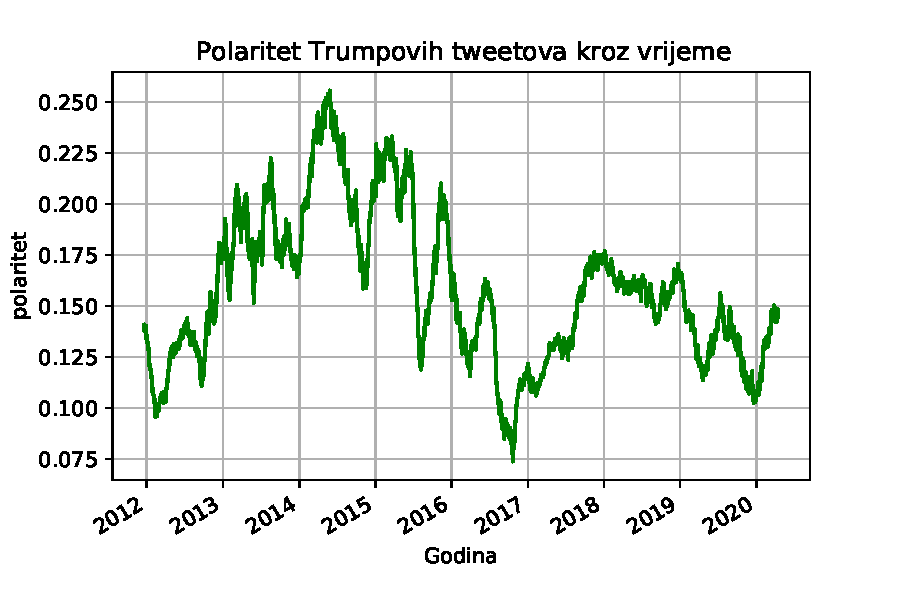
\includegraphics[scale=0.9]{../rad/slike/polaritet.pdf}
	\end{figure}
\end{frame}

\begin{frame}[fragile]
	\frametitle{Rezultat}
	\begin{figure}
		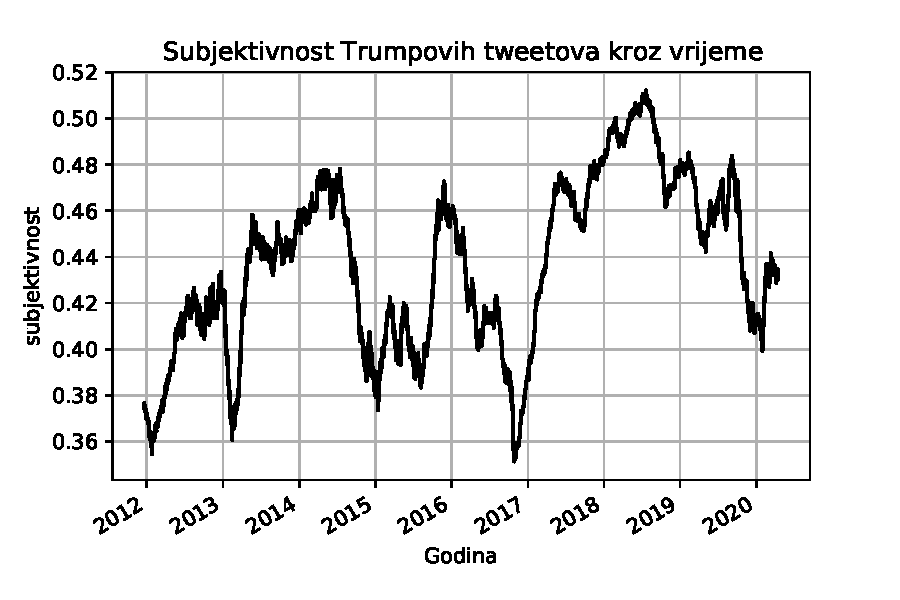
\includegraphics[scale=0.9]{../rad/slike/subjektivnost.pdf}
	\end{figure}
\end{frame}


\begin{frame}[fragile]
	\frametitle{Zaključak analize \textit{tweetova}}
	Zaključak: Trump se uozbiljio za vrijeme preizborne kampanje.
\end{frame}


\section{Zaključak}
\begin{frame}[fragile]
	\frametitle{Zaključak}
	\texttt{TextBlob} je:
	\begin{itemize}
		\item snažan alat
		\item fleksibilan alat
		\item jednostavan uvod u NLP
	\end{itemize}



\end{frame}

\end{document}


